\def\currentRootFolder{chapter/sensitivityStudyWithPreliminaryKatrinElossModel}
\def\currentFigureFolder{\currentRootFolder/fig}

\chapter{Sensitivity Study Using an Empirical Energy Loss Model Derived from KATRIN Data for Electrons Scattering Inelastically off Deuterium}
\label{sec:katrinEloss}
A quantitative accurate description of the scattering processes of $\upbeta$ electrons within KATRIN's gaseous tritium source is of crucial importance for the neutrino-mass-sensitivity goal. In modeling the corresponding effects, the energy loss function (see section~\ref{sec:intSpecModelResponseEloss}) plays an important role. The KATRIN Design Report states that the precision of the energy loss functions from literature is not sufficient for the KATRIN-sensitivity goal. It was planned to deduce a sufficiently accurate model from data taken at KATRIN~\cite{Angrik:2005ep}. In that regard, a preliminary model has successfully been established for electrons scattering off deuterium molecules based on data taken in October 2018 by a dedicated subgroup of the KATRIN collaboration. In the following, this model is referred to as the ``KATRIN model'' or the ``KATRIN energy loss model''. This preliminary energy loss model has partially-improved uncertainties with respect to the model from literature by~\cite{Aseev2000}, which was used in many previous works with regard to KATRIN~\cite{Groh2015,Kleesiek2014, Kleesiek2019, SeitzM2019}. In the following, the latter model is referred to as the ``Aseev model'' after the primary author of the corresponding publication~\cite{Aseev2000}. Additionally, the KATRIN model exhibits features not present in the Aseev model, but motivated by data (see section~\ref{sec:katrinElossModel} and figure~\ref{fig:katrinElossElossModel}). Within the scope of this thesis, the impact on KATRIN's sensitivity by the exchange of the Aseev model for the KATRIN model was studied. Therefore, this chapter is structured as follows: Section~\ref{sec:katrinElossConcept} presents the general idea of this study. Section~\ref{sec:katrinElossModel} outlines the KATRIN model. Section~\ref{sec:katrinElossValidity} discusses the scope of the validity of this study; for example what is expected of the comparison of a model for electrons scattering off deuterium and another model for scattering off tritium. Section~\ref{sec:katrinElossStatistics} introduces the applied statistical tools. Section~\ref{sec:katrinElossModelResults} lists and discusses the results. And section~\ref{sec:katrinElossModelOutlook} concludes and offers an outlook.

\section{Motivation and Introduction}
\label{sec:katrinElossConcept}
As the energy loss function is a source of systematic uncertainties within neutrino mass inference, it is of importance to provide early feedback to the team that measures it. Beyond that, the implementation of the required statistical tools into the available software frameworks is of general interest as the approach taken in the scope of this thesis may be applied to other model uncertainties, not only to the ones stemming from the energy loss function.

For the conducted sensitivity study, KATRIN neutrino mass measurements were simulated assuming a neutrino mass of~\SI{0}{eV} and using the KATRIN energy loss model. The further simulation parameters are based on the KATRIN Design Report~\cite{Angrik:2005ep}. A confidence interval for the neutrino mass was deduced using the profile-likelihood method as described in the subsequent section~\ref{sec:katrinElossStatisticsProfileLikelihood}. This enables the treatment of the model uncertainties and their correlations as nuisance parameters. This approach is repeated for the Aseev model to enable a comparison. Furthermore, the case with all parameters of the KATRIN model fixed to their best estimates is also evaluated as a further comparison.

\section{The Empirical KATRIN Energy Loss Model}
\label{sec:katrinElossModel}
\begin{figure}[h!]
	\centering
	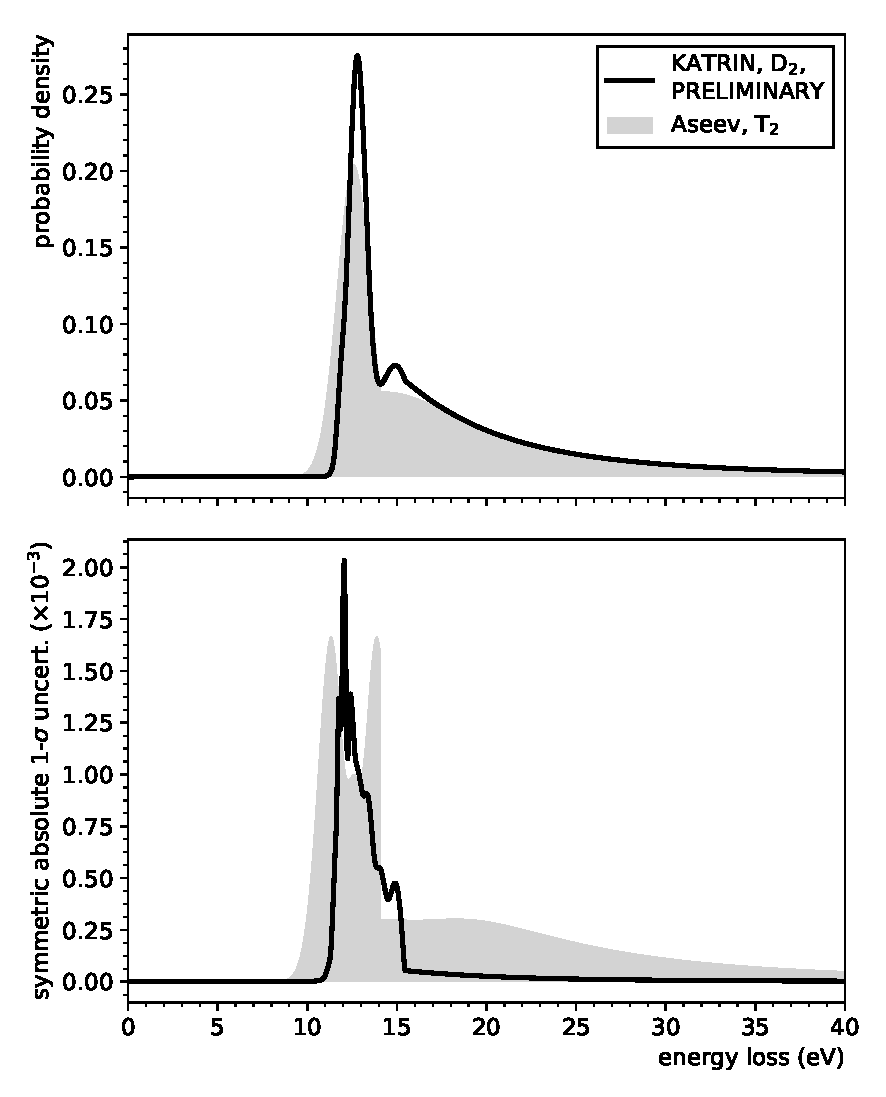
\includegraphics[width=\textwidth]{\currentFigureFolder/KATRINandAseevElossModel}
	\xcaption{The preliminary empirical KATRIN energy loss model for electrons scattering off deuterium molecules}{The preliminary empirical KATRIN energy loss model for electrons scattering off deuterium molecules.}{The black line shows the KATRIN energy loss model as established by a dedicated subgroup of the KATRIN collaboration for electrons scattering off deuterium molecules (KATRIN model). The corresponding model for scattering off tritium molecules as established by~\cite{Aseev2000} (Aseev model) is shown for comparison as a shaded area. (That the latter is plotted as area instead of as a line solely serves readability as the two functions overlap strongly.) The top panel shows the probability densities of the energy loss and the bottom panel shows the corresponding absolute symmetric 1-$\sigma$ uncertainties. The uncertainties were obtained through uncertainty propagation via derivatives from the uncertainties of the model parameters (see figure~\ref{fig:intSpecModelAseevEloss} for the Aseev model and appendix~\ref{sec:appendixKatrinElossElossModelParams} for the KATRIN model). Correlations are respected for the KATRIN model. However, there are no published correlations for the Aseev model. The KATRIN model shows particularly improved uncertainties in the ionization tail region in comparison to the Aseev model. (KATRIN model adapted from~\cite{Hannen2019_1}.)}
	\label{fig:katrinElossElossModel}
\end{figure}
The presented KATIRIN energy loss model is a phenomenological description fitted to data taken at the KATRIN experiment in October 2018. It was established by a dedicated subgroup of the KATRIN collaboration. The model is outlined in the following.

\subsection{Description}
Figure~\ref{fig:katrinElossElossModel} shows the KATRIN model in comparison to the Aseev model. They are not expected to be fully compatible within their uncertainties as they describe the scattering off two different hydrogen isotopologues. For a comparison of the presented KATRIN model with an energy loss model for deuterium from literature, the reader is referred to~\cite{Rodenbeck2019}. Furthermore, the parametrization of the KATRIN model comprises a second peak for excitation and molecular dissociation of deuterium. As the KATRIN model is still in its early stages, this work refrains from a detailed physical interpretation and instead focuses on uncertainty propagation. For a more detailed physical interpretation, the reader is referred to the KATRIN documents~\cite{Rodenbeck2019,Hannen2019_1,Hannen2019_2}. With respect to the uncertainties, the KATRIN model shows an improved uncertainty in the ionization tail and also in large parts of the excitation peak. How this propagates within neutrino mass inference is investigated in this chapter.

\subsection{Parametrization}
In the preceding section~\ref{sec:intSpecModelResponseEloss}, the energy loss function $f_1(\epsilon)$ is introduced. It denotes the probability density for an energy $\epsilon$ that an electron loses when scattering once (inelastically in the current context). The KATRIN model is such an energy loss function. It can be divided into two parts. The first part is the phenomenological description of the excitation peak region by the sum of three scaled Gaussian distributions $\mathcal{N}$. This part $\d\sigma_\mathrm{exit}^\mathrm{phen}/\d \epsilon$  can be described by nine parameters $\nuisanceParamVec_\mathrm{eloss}$ which comprise the three scales $A_i$, means $m_i$ and standard deviations $s_i$ ($i \in \{1,2,3\}$) of the three Gaussian distributions~\cite{Hannen2019_2}
\newcommand{\katrinElossPhen}[1]{
	\frac{
		\d\sigma_\mathrm{exit}^\mathrm{phen}\giventhat*{#1}{\nuisanceParamVec_\mathrm{eloss}}
	}{
		\d \epsilon
	}
}
\begin{align}
\label{eq:katrinElossElossModelParams}
\nuisanceParamVec_\mathrm{eloss} &= 
\transp{\left(
	A_1, m_1, s_1, 
	A_2, m_2, s_2, 
	A_3, m_3, s_3
	\right)} \\
\katrinElossPhen{\epsilon} &=
\sum_{i=1}^3 A_i \cdot \mathcal{N}(\epsilon, \mu=m_i, \sigma=s_i)
\fullstop
\end{align}
The second part, the ionization tail, follows a modified version of the binary-encounter-dipole (BED) model. For a full formula, the reader is referred to~\cite{Kim1994}. Here, this part will be denoted
\newcommand{\katrinElossBDE}[1]{
	\frac{
		\d \sigma_\mathrm{ion}^\mathrm{BED}(#1)
	}{
		\d \epsilon
	}
}%
\newcommand{\ionEnergyDeu}{E_\mathrm{ion,D_2}}%
\begin{equation}
	\katrinElossBDE{\epsilon}
	\fullstop
\end{equation}%
The BED model is valid for hydrogen molecules. Therefore, it depends on the ionization energy of hydrogen. The corresponding value was exchanged for the one of deuterium $\ionEnergyDeu=\SI{15.467}{eV}$~\cite{Shiner1993}. Whether further modifications with regard to the difference in isotopologues are necessary is currently under investigation. Furthermore, the constant normalization factor of the BED model was removed for the following reason: The transition between the two parts, the phenomenological peak and the BED tail, is introduced at the ionization energy of deuterium $\ionEnergyDeu$. In order for the transition to be continuous, a scaling factor for the ionization tail is introduced
\begin{equation}
c = \left.	
	\left(
		\katrinElossPhen{\ionEnergyDeu}
	\right)
\middle/
	\left(
		\katrinElossBDE{\ionEnergyDeu}
	\right)
\right.
\fullstop
\end{equation}
Then, the full parametrization for the KATRIN model reads~\cite{Hannen2019_1}
\begin{equation}
	f_1^\mathrm{KATRIN}
	\giventhat*{\epsilon}{\nuisanceParamVec_\mathrm{eloss}} = 
	\begin{cases}
	\katrinElossPhen{\epsilon}
	&\text{ if } \epsilon \leq E_\mathrm{ion,D_2} \\
	\vphantom{.} & \\
	c \cdot \katrinElossBDE{\epsilon} 
	&\text{ if } \epsilon > E_\mathrm{ion,D_2}
	\end{cases}
	\fullstop
\end{equation}

\subsection{Nuisance Parameters}
The uncertainties of the KATRIN model as evaluated at the time of writing this thesis can be divided into two sets: The KATRIN model itself comprises nine parameters. However, it was obtained in a 15-parameter fit. The other six fit parameters are correlated with the parameters of the KATRIN model and hence are not necessarily negligible with regard to uncertainties. In the scope of this thesis, they were incorporated in the statistical treatment of the uncertainties. Whether they may be neglected in future studies needs further investigation. 

For a detailed description of the full fit of the KATRIN model to the recorded data, the reader is referred to~\cite{Hannen2019_1}, but a description of the essentials is given in the following. An overview of the used data sets is required in order to describe the further six fit parameters. Four integral spectra were recorded analogously to the described integral $\upbeta$ spectrum in chapter~\ref{sec:intSpecModel}, but with the electron gun (see section~\ref{sec:katrinExpSetupRearSection}) as electron source instead of tritium. For each data set a different deuterium column density (see section~\ref{sec:katrinExpSetupWGTS}) was set in the \gls{wgts}: \SI{0}{\percent}, \SI{15}{\percent}, \SI{50}{\percent}, \SI{100}{\percent} of the nominal column density of $\rho d = \SI{5e17}{molecules/cm^2}$. The fit model for the \mbox{\SI{15}{\percent}-measurement} was rescaled with respect to the other measurements because the respective data set underwent a different preprocessing than the others. The corresponding scaling factor $N_{\mathrm{int},15}$ was a free fit parameter. A further scaling factor $N_\mathrm{K}$ for the KATRIN model was introduced in the fit as a free parameter in order for the whole KATRIN model to keep its properties of a probability density and integrate to unity. Additionally, a 5th data set recorded at $\SI{15}{\percent}$ column density in a time-of-flight mode~\cite{Bonn1999} was fitted simultaneously. For each data set, a different expected scattering count $
\mu_{\mathrm{tof},15}, 
\mu_{\mathrm{int},15},  
\mu_{\mathrm{int},50},  
\mu_{\mathrm{int},100}$ (see equation~\ref{eq:intSpecModelExpectedScatteringCount}) was fitted, which adds four further parameters (there is no scattering for the $\SI{0}{\percent}$ measurement). In summary, the additional parameters in the fit of the KATRIN model are
\begin{equation}
\label{eq:katrinElossElossModelExtendedParams}
	\nuisanceParamVec_\mathrm{eloss+} = 
	\transp{\left(
		N_\mathrm{K},
		\mu_{\mathrm{tof},15},
		\mu_{\mathrm{int},15}, 
		\mu_{\mathrm{int},50}, 
		\mu_{\mathrm{int},100},
		N_{\mathrm{int},15}
		\right)}
	\fullstop
\end{equation}
The best best-fit values, the standard deviations and the correlation matrix of the full 15-parameter set ($\nuisanceParamVec_\mathrm{eloss}$ and $\nuisanceParamVec_\mathrm{eloss+}$) can be found in appendix~\ref{sec:appendixKatrinElossElossModelParams}. The aim of this chapter is to study the impact of the model uncertainties from these 15 parameters on KATRIN's sensitivity to the neutrino mass.

\section{Scope of the Presented Analysis}
\label{sec:katrinElossValidity}
This section lists considerations that should be kept in mind with regard to the study presented in this chapter.

First, it should be noted that the KATRIN model as presented is still preliminary and may be subject to change because the analysis of recent measurements is still ongoing.

Furthermore, during a neutrino mass measurement, the nominal tritium purity in the~\gls{wgts} is planed to be above~\SI{95}{\percent}~\cite{Angrik:2005ep}. Here, an energy loss model for deuterium is used. Two different, but similar energy loss models are expected for the two different gas species (compare~\cite{Abdurashitov2017} and~\cite{Aseev2000}). Within the scope of this thesis, the impact on KATRIN's sensitivity from the reduction of uncertainties on the energy loss model are of primary interest. As long as the KATRIN model for scattering off deuterium molecules is sufficiently similar to the model for scattering off tritium molecules, it is a plausible approach to use it for simulations of KATRIN neutrino mass measurements (for the similarity, see figure~\ref{fig:katrinElossElossModel}). In that regard, the results for KATRIN's sensitivity derived in this chapter are expected to be meaningful, at least as a proof of concept.

Furthermore, the KATRIN model does not yet incorporate systematic uncertainties. Corresponding efforts for their incorporation are made at the time of writing this thesis. A future version of the KATRIN model may exhibit larger uncertainties than the version used in this thesis.
\FloatBarrier
\def\currentRootFolder{chapter/sensitivityStudyWithPreliminaryKatrinElossModel/statisticalPrerequisites}
\def\currentFigureFolder{\currentRootFolder/fig}
\newcommand{\elecIndex}{\mathrm{e}}

\newcommand{\Bsource}{B^j_\mathrm{S}}
\newcommand{\BsourceAvg}{B_\mathrm{S}}
\newcommand{\zSource}{z_\mathrm{S}}
\newcommand{\thetaSource}{\theta_\mathrm{S}}
\newcommand{\thetaSourceAvg}{\theta_\mathrm{S}}
\newcommand{\Esource}{E_\mathrm{S}}
\newcommand{\Usource}{U^j_\mathrm{S}}
\newcommand{\gammaSource}{\gamma_\mathrm{S}}


\newcommand{\Bps}{B_\mathrm{PS2}}
\newcommand{\Bana}{B_\mathrm{A}}
\newcommand{\Bpinch}{B_\mathrm{P}}
\newcommand{\Bmax}{B_\mathrm{max}}
\newcommand{\Bmin}{B_\mathrm{min}}

\newcommand{\thetaMax}{\theta_\mathrm{max}}
\newcommand{\Esur}{E_\mathrm{sur}}
\newcommand{\detEff}{\epsilon_\mathrm{det}}
\newcommand{\macefilterwidth}{\Delta \mathcal{E}^j(\thetaS^j)}

\newcommand{\EtransPure}{E^j_\mathrm{tr}}
\newcommand{\Etrans}{\EtransPure(qU,\Esource,\thetaSource)}
\newcommand{\thetaTransPure}{\theta^j_\mathrm{tr}}
\newcommand{\thetaTrans}{\thetaTransPure(\Esource,qU)}

\newcommand{\As}{A_\mathrm{S}}
\newcommand{\Rbg}{R_\mathrm{bg}}


\newacronym{standardmodel}{SM}{Standard Model of Particle Physics}
\newacronym{lep}{LEP}{Large Electron Positron Collider}
\newacronym{ssm}{SSM}{standard solar model}

\section{Statistical Prerequisites}
\label{sec:katrinElossStatistics}
\subsection{Nuisance Parameters and the Profile Likelihood Method}
\label{sec:statMethodsProfileLikelihood}
Apart from the  parameters of interest $\paramVec$ (usually the squared neutrino mass), the KATRIN likelihood depends on further so-called nuisance parameters $\nuisanceParamVec$ (e.\,g. the background rate). The dimensionality may pose difficulties when deriving a confidence region for the combined parameter set. Furthermore, as indicated by the naming conventions, the dimensions of the nuisance parameters in the confidence region are not of interest. Hence, in order to derive a confidence interval with restricted dimensions, a test statistic, similar to the one in equation~\ref{eq:statMethodsLikelihoodRatio}, but that solely depends on the parameters of interest, has to be found. The following paragraph outlines, how a corresponding test statistic can be constructed using the profile likelihood method.

A corresponding derivation may start with the definition of the profile likelihood: The profile likelihood only depends on the parameters of interest $\paramVec$. Its values correspond the likelihood values evaluated at $\paramVec$ in the dimensions of the parameter of interest and maximized in the dimensions of the nuisance parameters~\cite{ReviewOfParticlePhysics}
\begin{equation}
\profLikelihood(\paramVec) = 
L(\paramVec, \hat{\hat{\nuisanceParamVec}}(\paramVec))
\comma
\end{equation}
where the double-hat indicates the maximization respectively the profiling. Also, the profile likelihood ratio can be defined~\cite{ReviewOfParticlePhysics}
\begin{equation}
\label{eq:statMethodsProfileLikelihoodRatio}
\lambda_\mathrm{p}(\paramVec) = 
\frac{\profLikelihood(\paramVec)}{\profLikelihood(\hat{\paramVec})}
\fullstop
\end{equation}
According to Wilks’ theorem~\cite{wilks1938}, the distribution of $-2\ln\lambda_\mathrm{p}(\hat{\paramVec})$, where $\hat{\paramVec}$ is the \gls{mle}, approaches a $\chi^2$ distribution in the limit of a large data sample, independent of the values of the nuisance parameters $\nuisanceParamVec$~\cite{ReviewOfParticlePhysics}. Hence, the profile likelihood ratio offers a test statistic, from which a confidence interval for the parameters of interest can be derived.

In application to a KATRIN neutrino mass measurement, the introduced formalism can be summarized as follows: The profile likelihood~\eqref{eq:statMethodsProfileLikelihoodRatio} is a measure (test statistic) for whether a hypothesized squared neutrino mass has to be rejected given the KATRIN data. Furthermore, analogously to section~\ref{sec:statMethodsUncertaintyIntervalsConfidence}, this allows for the derivation of a confidence interval for the squared neutrino mass. It should be noted, however, that this method requires an extrapolation of the likelihood to nonphysical negative squared neutrino masses~\cite{Kleesiek2014}.


\subsection{Sensitivity from  the Profile Likelihood Method}
In the scope of this thesis, the sensitivity on the neutrino mass is evaluated using the profile likelihood method (section~\ref{sec:statMethodsProfileLikelihood}) in order to account for nuisance parameters and especially their correlations. The profile likelihood method was also used in~\cite{Kleesiek2014} for a KATRIN standard 4-parameter fit (section~\ref{sec:statMethodsProfileLikelihood}). The obtained value for $\statUncert$ is plotted and can be extracted to be between \SIrange[range-phrase=--]{0.0155}{0.0165}{eV^2} which is in agreement with the result $\statUncert=\SI{0.0162}{eV^2}$ from ensemble testing (see table~\ref{tab:statMethodsSensitivityFromEnsembleTests}). ``In case of the standard 4 parameter fit, the confidence intervals calculated from ensemble tests are in very good agreement with alternative methods [...], including likelihood ratio intervals (profile likelihood method)'' Kleesiek, page 160, profile likelihood, optimized mtd, uncertainty on suqred mnu $0.01494 eV^2$.



\subsection{Combination of Commissioning and Neutrino Mass Measurements}
If two measurements share a set of parameters $\paramVecShared$, but have additionally an individual set of parameters $\paramVec_1$ and $\paramVec_2$ and different sets of observations a combined likelihood is given by the product of the single likelihoods $L_1$ and $L_2$
\begin{equation}
-2\ln L(\paramVecShared, \paramVec_1, \paramVec_2) =  
-2\ln L_1(\paramVecShared, \paramVec_1)
-2\ln L_2(\paramVecShared, \paramVec_2)
\fullstop
\end{equation}
In the case of KATRIN the first measurement could be sensitive to the neutrino mass whereas say the second measurement could have been a calibration using the electron gun and be sensitive to parameters of the response function \eqref{eq:SSCresponse}. Combining both likelihoods would incorporate the uncertainties on the parameters of the response function in the neutrino mass determination. Currently, no software framework exists that allows the construction of combined likelihoods of KATRIN neutrino mass and calibration measurements. Instead the following approximation can be made. The calibration measurement is evaluated independently and one obtains estimates $\hat{\paramVec}_\mathrm{s,2}$, and an estimated covariance matrix $\hat{V}_\mathrm{s,2}$ for all components of $\paramVecShared$ that the calibration measurement is sensitive to. These can in turn be used to approximate the likelihood $L_2$ at least in the dimension of $\paramVecShared$. A choice that stands to reason for the approximation of $L_2$ is a multivariate Gaussian distribution. For the purpose of parameter inference through minimization $-2\ln L_2$ needs only to be accurately approximated around its minimum. The choice of a multivariate Gaussian distribution corresponds a symmetric approximation of $-\ln L_2$ around its minimum by a parabola. The KATRIN likelihood for a combination of a neutrino mass and a calibration measurement then reads
\begin{equation}
\begin{split}
\label{eq:penalizedLikelihood}
-2\ln L(\paramVecShared, \paramVec_1, \paramVec_2) &\approx
-2\ln L^\prime(\paramVecShared, \paramVec_1) \\ &=
\underbrace{
	\chi^2(\paramVecShared, \paramVec_1)
	\vphantom{(\paramVecShared - \hat{\paramVec}_\mathrm{s,2})^{\mathsf{T}}}
}_{(1)}
+
\underbrace{
	(\paramVecShared - \hat{\paramVec}_\mathrm{s,2})^{\mathsf{T}}
	\hat{V}_\mathrm{s,2}^{-1}
	(\paramVecShared - \hat{\paramVec}_\mathrm{s,2})
}_{(2)} +\; 
\mathrm{ constants}\\ &=
\chi^2(\paramVecShared, \paramVec_1) 
-2\ln \mathcal{N}(\paramVecShared, \hat{\paramVec}_\mathrm{s,2}, \hat{V}_\mathrm{s,2}^{-1}) +
\mathrm{ constants}
\end{split}
\end{equation}
Here, $(1)$ is the chi-square expression \eqref{eq:katrinChi2} where the $\paramVecShared$ and $\paramVec_1$ can be written as one combined parameter vector $\paramVec$ for a neutrino mass measurement. And $(2)$ resembles the negative log likelihood of the calibration measurement approximated by a multivariate Gaussian distribution. Terms having a form like $(2)$ are also sometimes called ``pull terms'' or ``likelihood penalties''. In the minimization process they ``pull'' the parameters $\paramVecShared$ towards $\hat{\paramVec}_\mathrm{s,2}$ respectively ``penalize''/increase the negative log likelihood if $\paramVecShared$ and $\hat{\paramVec}_\mathrm{s,2}$ differ.


\newcommand{\CombLmax}{-2\ln L(\hat{\paramVec}_\mathrm{s}, \hat{\paramVec}_1)}
The chi-square term $(1)$ is a sum of $n$ standard normal distributed random variables. Hence, as discussed, a likelihood only composed of the chi-square term $(1)$ offers a goodness-of-fit criteria via the the Pearson chi-square statistic. Note that for the combined likelihood this criteria might not hold. Two special cases can be considered where the chi-square characteristics hold approximately: First, the neutrino mass measurement, term $(1)$, is not sensitive to the shared parameters $\d \chi^2(\paramVecShared, \paramVec_1) /\d \paramVecShared \approx 0$. Then the \gls{mle} for the shared parameters will match the \gls{mle} by the calibration measurement $\hat{\paramVec}_\mathrm{s} = \hat{\paramVec}_{\mathrm{s},2}$ and term $(2)$ will be 0. The combined likelihood evaluated at the \gls{mle} $\CombLmax$ then follows a chi-square distribution with $n-\dim\paramVec_1-\dim\paramVecShared$ degrees of freedom. Second, if the neutrino mass measurement is sensitive to some shared parameters $\d \chi^2(\paramVecShared, \paramVec_1) /\d \paramVecShared \neq 0$, then one might argue, that term $(2)$ evaluated at the \gls{mle} $\hat{\paramVec}_\mathrm{s} \neq \hat{\paramVec}_{\mathrm{s},2}$ is a sum of standard normal distributed random variables. If this holds, the combined likelihood evaluated at the \gls{mle} $\CombLmax$ follows a chi-square distribution with $n-\dim\paramVec_1$ degrees of freedom.


For example, a standard KATRIN 3-year neutrino mass measurement is not at all sensitive to parameters of the energy loss function \eqref{eq:nonAveragedResponse}. Hence, adding a corresponding term $(2)$ from a designated energy loss measurement will not influence the chi-square characteristics. However, a standard KATRIN neutrino mass measurement is even after a short measurement time sensitive to the gas column density \eqref{eq:columnDensity}. Adding a corresponding term $(2)$ from (a naturally more sensitive) monitoring measurement would influence the   


\todo{Add plots from ensemble test that proof statements.}

\subsection{Extension of the KaFit Software Framework}
\label{sec:statLikelihoodExtImpl}
The likelihood $L(\paramVec)$ can be multiplied by a function $g(\paramVec)$
\begin{equation}
\label{eq:likelihoodExtension}
-2\ln L^\prime(\paramVec) = -2\ln L(\paramVec) -2\ln g(\paramVec)
\fullstop
\end{equation}
This procedure may have different interpretations and usage scenarios. E.g. a comparison with \eqref{eq:posterior} shows, if $g$ is a prior probability distribution, $L^\prime$ becomes a non-normalized posterior distribution that can be used in a Bayesian analysis. A further interpretation is given in section \ref{sec:combinationOfMeasurements}.
\label{sec:combinationOfMeasurements}

KaFit allowed to choose $g$ in \ref{eq:likelihoodExtension} as a product of one-dimensional Gaussian distributions. Within this thesis the software was extended to allow products of other functions. Three function types were explicitly made available through a configuration file.
\begin{enumerate}
	\item A reimplementation of a one-dimensional Gaussian distribution: The reimplementation was necessary to conveniently enable the combination of function types.
	\item A multivariate Gaussian distribution: This enables the treatment of uncertainties quantified by calibration or monitor measurements as described in section \ref{sec:combinationOfMeasurements}. It can also be used as a prior distribution in a Bayesian analysis. Particularly, correlations can be respected.
	\item A one-dimensional probability density, that is constant in the square root of a parameter, if it is positive and 0 otherwise:
	\begin{equation}
		g(\theta) =
		\begin{cases}
		0 &\text{ if } \theta \leq 0 \\
		\text{constant} \cdot \frac{1}{\sqrt{\theta}} &\text{ if } \theta > 0
		\end{cases}
		\fullstop
	\end{equation}
	 This can be used as a uniform prior on the neutrino mass ($\theta=m_\nu^2$). Formerly, it was only possible to use a uniform prior on the squared neutrino mass. A derivation of the form of $g$ can be found in appendix \ref{sec:appStatisticPriorOnNu2}.
\end{enumerate}
An example on how to configure KaFit using the new feature is given in appendix \todo{Add appendix}.


\def\currentRootFolder{chapter/sensitivityStudyWithPreliminaryKatrinElossModel}
\def\currentFigureFolder{\currentRootFolder/fig}
\FloatBarrier
\section{Results}
\label{sec:katrinElossModelResults}
This section lists the results of the study on the impact from the uncertainties of the KATRIN model on KATRIN's sensitivity. The results are compared to the impact of the uncertainties from the Aseev model. The sensitivity study was conducted using a mathematical model of a KATRIN neutrino mass measurement as described in chapter~\ref{sec:intSpecModel} using a nominal configuration according to the KATRIN Design Report~\cite{Angrik:2005ep} with a neutrino mass of \SI{0}{eV} and a measurement time of three years. Correspondingly, the SSC and KaFit modules were used (see section~\ref{sec:statMethodsKaFitSSC}). The full configuration of the study can be found in appendix~\ref{sec:appendixKatrinElossSSCConfig}. The uncertainties of the KATRIN respectively the Aseev model were respected as described in section~\ref{sec:katrinElossStatisticsCombMeasurements} about the combination of a neutrino mass and a calibration measurement. The confidence interval for the squared neutrino mass was extracted via the profile-likelihood method as described in section~\ref{sec:katrinElossStatisticsProfileLikelihood}.

Section~\ref{sec:katrinElossModelResultsAsimov} presents the study using an Asimov data set. And section~\ref{sec:katrinElossModelResultsEnsemble} presents the same results as obtained through an ensemble test (for the relation of these two approaches see section~\ref{sec:katrinElossStatisticsAsimov}).
\subsection{Sensitivity from an Asimov Data Set}
\label{sec:katrinElossModelResultsAsimov}
\begin{figure}[t]
	\centering
	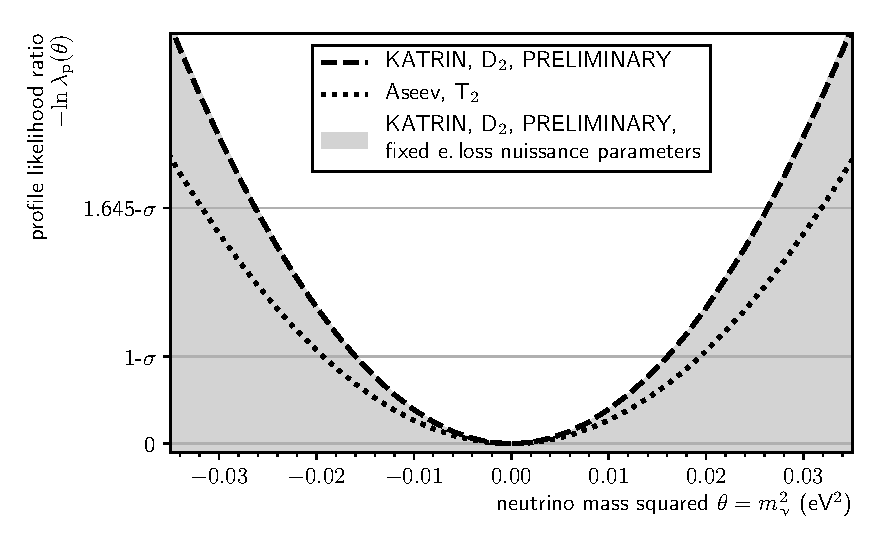
\includegraphics[width=\textwidth]{\currentFigureFolder/profileLikelihoodKATRINandAseev.pdf}
	\xcaption{Profile-likelihood ratio of a KATRIN measurement from an Asimov data set}{Profile-likelihood ratio of a KATRIN measurement  from an Asimov data set.}{The graph shows the profile-likelihood ratio $\lambda_\mathrm{p}$ for three different cases with different uncertainties: using the KATRIN model (dashed line), the Aseev model (dotted line) or the ``statistics only'' case (shaded area). For a description of the different cases, the reader is referred to the main text. (That the ``statistics only'' case is plotted as area instead of as a line solely serves readability because a line would overlap with the line for the KATRIN model.) The \gls{mle} recovers the true simulated neutrino mass of \SI{0}{eV} with a corresponding likelihood ratio of 0. The horizontal $s$-$\sigma$ lines are drawn at $s^2/2$ as per equation~\eqref{eq:statMethodsConfidenceContour}. Their intersections with $-\ln\lambda_\mathrm{p}$ mark the confidence intervals for the neutrino mass at \SI{68}{\percent} respectively \SI{90}{\percent} confidence level. The width of the two intervals indeed relate through the factor 1.645 due to the parabolic shape of $-\ln\lambda_\mathrm{p}$. It is apparent, that the uncertainties of the KATRIN model are negligible with respect to the ``statistics only'' case. The corresponding profile likelihoods are almost equal.}
	\label{fig:katrinElossResultsProfileLikelihood}
\end{figure}
The following three cases were investigated using an Asimov data set:\mynobreakpar
\begin{enumerate}
	\item The simulation- and fit-model use the KATRIN energy loss model, but it was assumed to be without uncertainties. In other words, only the four parameters of a nominal KATRIN-neutrino-mass fit (see section~\ref{sec:statMethodsStandardFit}) were treated as free parameters and the parameters of the KATRIN energy loss model were fixed to their best estimates. In the following, this is referred to as the ``statistics only'' case.
	\item The simulation- and fit-model use the KATRIN energy loss model, and all its parameters were treated as free in order to incorporate the uncertainties of the KATRIN model, which results in a 19-parameter fit.
	\item The simulation- and fit-model use the Aseev model, and all its parameters were treated as free in order to incorporate the uncertainties of the Aseev model, which results in a nine-parameter fit.
\end{enumerate}
Figure~\ref{fig:katrinElossResultsProfileLikelihood} shows the corresponding profile-likelihood ratios and table~\ref{tab:katrinElossModelResultsAsimov} lists the extracted confidence intervals and obtained sensitivities. The ``statistics only'' case can be compared to the results listed in table~\ref{tab:statMethodsSensitivityFromEnsembleTests}. Here, a $\sim\SI{4e-4}{eV^2}$ smaller statistical uncertainty on the squared neutrino mass is obtained compared to the results by~\cite{Kleesiek2014, Hoetzel2012}. This is mainly due to the fact, that in the study presented in this chapter a detection efficiency of \SI{95}{\percent} was used, whereas the other works used~\SI{90}{\percent}.

Under the restrictions listed in section~\ref{sec:katrinElossValidity}, the following conclusions can be drawn:
\begin{itemize}
	\item Using the KATRIN model at its current stage yields an improvement of~\SI{10}{meV}  in sensitivity to the neutrino mass compared to using the Aseev model.
	\item The uncertainties stemming from the KATRIN model are negligible with respect to the statistical uncertainty.
	\item The logarithm of the profile-likelihood ratio has a parabolic shape, which translates to a Gaussian shape for the likelihood. This hints at the applicability of  Wilks' theorem to verify the usage of the profile-likelihood method and Walt's theorem to enable the usage of an Asimov data set. It also justifies the usage of the factor $1.645$ to convert a confidence interval of~\SI{68}{\percent} confidence level into one of~\SI{90}{\percent}.
\end{itemize}

\begin{table}[t]
	\centering
	\xcaption{Neutrino mass confidence intervals and sensitivities obtained from an Asimov data set}{Neutrino mass confidence intervals and sensitivities obtained from an Asimov data set.}{The table lists values that can be extracted from the profile-likelihood ratio depicted in figure~\ref{fig:katrinElossResultsProfileLikelihood} for the three conducted studies: the ``statistics only'' case and respecting the uncertainties from the KATRIN and the Aseev model. Listed are the lower bound of the confidence interval (\SI{60}{\percent} C.L.) on the squared neutrino mass $l(\nuMass^2)$, the upper bound $u(\nuMass^2)$, half the width of the interval $\sigma_\mathrm{tot}(\nuMass^2)$ and KATRIN's sensitivity on the neutrino mass as per equation~\eqref{eq:statMethodsSensitivity}. For the calculation of the sensitivity an additional systematic budget of $\SI{0.017}{eV^2}$ was included (see section~\ref{sec:statMethodsSensitivtyFromEnsemble}).}
	\begin{tabular}{lrrrr}
		\toprule
		\makecell[tr]{} &
		\makecell[tr]{$l(\nuMass^2)$ \\ (\SI{e-2}{eV^2})} & 
		\makecell[tr]{$u(\nuMass^2)$ \\ (\SI{e-2}{eV^2})} & 
		\makecell[tr]{$\sigma_\mathrm{tot}(\nuMass^2)$ \\ (\SI{e-2}{eV^2})} &
		\makecell[tr]{$S_{\nuMass}(\SI{90}{\percent})$ \\ (\SI{}{meV})}  
		\\
		\hline
		``statistics only'' & -1.586 & 1.592 & 1.589 & 196 \\
		KATRIN model & -1.598 & 1.604 & 1.601 & 196 \\
		Aseev model & -1.931 & 1.939 & 1.935 & 206 \\
		\bottomrule
	\end{tabular}
	\label{tab:katrinElossModelResultsAsimov}
\end{table}

\subsection{Cross-Check and Extension of the Asimov Data Set via Ensemble Testing}
\label{sec:katrinElossModelResultsEnsemble}
An ensemble of 4046 KATRIN neutrino mass measurements with a true neutrino mass of~\SI{0}{eV} was simulated using the KATRIN energy loss model and incorporating its uncertainties in the same manner as for the Asimov data set described in the last section~\ref{sec:katrinElossStatisticsAsimov}. Several aspects were investigated as listed below:

\paragraph{Test of Coverage}
The extraction of a confidence interval via the profile-likelihood method as done in the previous section~\ref{sec:katrinElossStatisticsAsimov} for the Asimov data set should per construction yield a coverage probability of \SI{68.2}{\percent}. But if all conditions are met for this to hold has to be justified. Either a theoretical argument can be given or it can simply be put to the test. In the scope of this thesis, the approach per test was chosen. In other words, \SI{68.2}{\percent} of the obtained confidence intervals in the conducted ensemble test should cover the true simulated neutrino mass of~\SI{0}{eV}. The obtained coverage is \SI{67.6}{\percent} as illustrated in figure~\ref{fig:katrinElossResultsCoverage}. The slight undercoverage on the $10^{-3}$ scale may stem from a limited ensemble test size. The difference is negligible within the typical rounding scheme to integer values for percentages in confidence levels.

\paragraph{Chi-Square Characteristics}
The combined likelihood of a neutrino mass and a calibration measurement evaluated at the \gls{mle} $-2\ln L(\hat{\paramVec})$ might not follow the chi-square statistic as mentioned in section~\ref{sec:katrinElossStatisticsCombMeasurements}. Figure~\ref{fig:katrinElossStatisticsChi2} shows the obtained distribution of $-2\ln L(\hat{\paramVec})$ in the conducted ensemble test. An \gls{mtd} with 41 retarding potentials was used. Hence, there are 41 summands in the likelihood for the KATRIN neutrino mass measurement. In the combined likelihood, there are additional 15 summands to approximate the likelihood of the measurement of the KATRIN energy loss model. In total there are 19 fit parameters, four for the nominal KATRIN neutrino mass fit (see section~\ref{sec:statMethodsStandardFit}) and 15 in order to incorporate the uncertainties of the KATRIN model. Thus, the hypothesis stands to reason that the obtained distribution follows a chi-square distribution with $41+15-19=37$ degrees of freedom. A corresponding Kolmogorov–Smirnov test yields a $p$-value of $p=\SI{6e-6}{}$. In other words, this hypothesis has to be rejected with a significance of $4\sigma$. Repeating the test for 38 respectively 39 degrees of freedom yields $p=\SI{0.14}{}$ respectively $p=\SI{1e-14}{}$. Hence, a chi-square distribution of 38 degrees of freedom may not be rejected. This is important because it means that the chi-square statistic can not necessarily be used as a measure for goodness-of-fit when incorporating the uncertainties of the KATRIN energy loss model into the neutrino mass inference in the way described in this thesis. Or, at least, one has to be careful about the choice of degrees of freedom. However, it must be emphasized that here the likelihood of the measurement of the KATRIN energy loss model is approximated by a multivariate normal distribution and does not fluctuate in the presented ensemble test. For the result to have full validity, the measurement of the KATRIN energy loss model has to be simulated along with the KATRIN neutrino mass measurement. This may be the aim of a future analysis.

\begin{figure}[th]
	\centering
	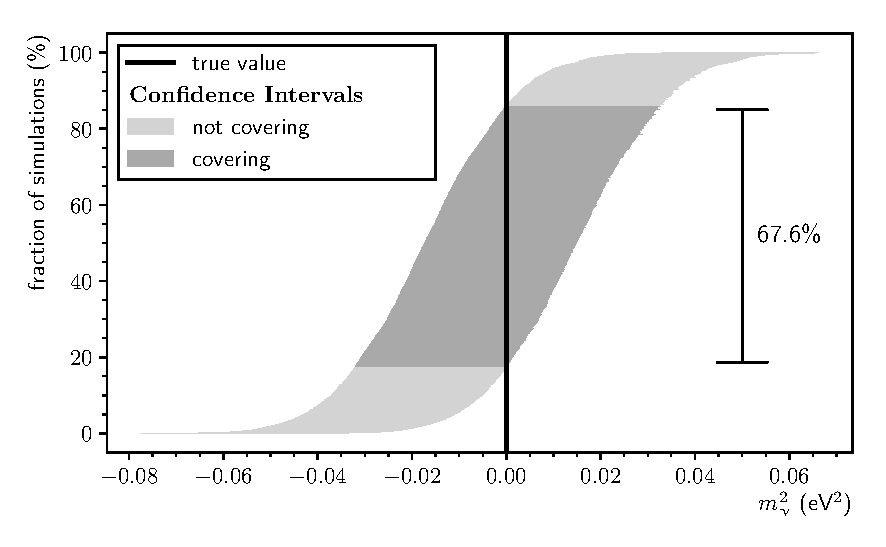
\includegraphics[width=\textwidth]{\currentFigureFolder/coverage.pdf}
	\xcaption{Test of coverage for the ensemble of confidence intervals obtained in the sensitivity study using the KARTRIN energy loss model}{Test of coverage for the ensemble of confidence intervals obtained in the sensitivity study using the KARTRIN energy loss model.}{The graph illustrates the coverage probability. An ensemble of 4046 KATRIN neutrino mass measurements with a true neutrino mass of~\SI{0}{eV} was simulated. For each simulated measurement a confidence interval was constructed using the profile-likelihood method. The obtained confidence intervals were sorted by their lower limit and plotted stacked which yields the gray band. The confidence intervals that cover the true value are depicted in dark gray, while the ones that do not cover the true value are depicted in light gray. In total~\SI{67.8}{\percent} coverage is obtained. In the limit of an infinite ensemble size, a coverage of~\SI{68.2}{\percent} would be expected per construction. It should also be noted, that there is little fluctuation in the width of the confidence intervals, which hints at the representative qualities of an Asimov data set.}
	\label{fig:katrinElossResultsCoverage}
\end{figure}

\paragraph{Representative Qualities of the Asimov Data Set}
The estimated mean and standard deviation of the distribution of the  confidence intervals (\SI{68}{\percent} C.L.) as obtained by the ensemble test is $\hat{\sigma}_\mathrm{tot}(\nuMass^2)=\SI{1.599\pm0.013e-2}{eV^2}$ in agreement with the one obtained through the Asimov data set in table~\ref{tab:katrinElossModelResultsAsimov}. Furthermore, the median confidence interval $\tilde{\sigma}_\mathrm{tot}(\nuMass^2)=\SI{1.598e-2}{eV^2}$ should recover the one of the Asimov data set~\cite{Cowan2011}, which is indeed the case on the \SI{e-5}{eV^2} level. This verifies the Asimov data set as representative for the study on the KATRIN energy loss model presented in this chapter.

\begin{figure}[t]
	\centering
	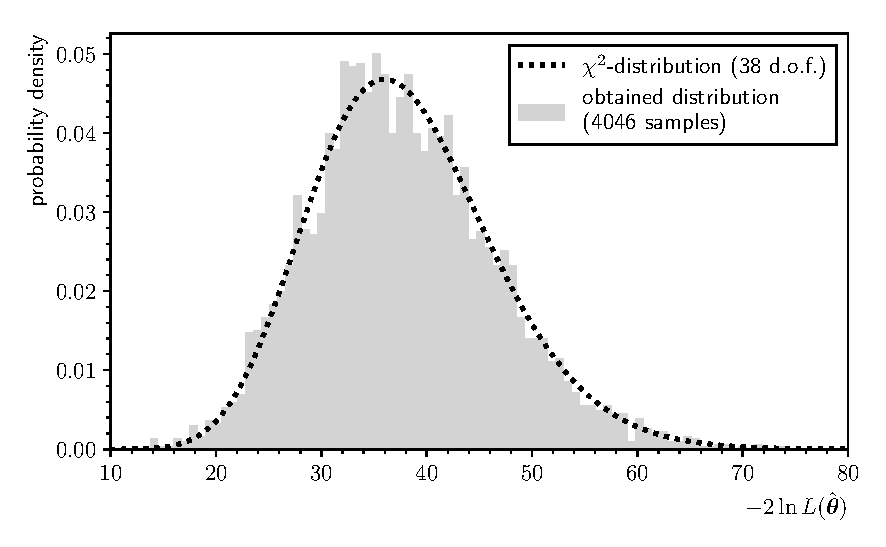
\includegraphics[width=\textwidth]{\currentFigureFolder/katrinElossChi2Distribution.pdf}
	\xcaption{Chi-square distribution for the simulated ensemble of neutrino mass measurements obtained in the sensitivity study using the KATRIN energy loss model}{Chi-square distribution for the simulated ensemble of neutrino mass measurements obtained in the sensitivity study using the KATRIN energy loss model.}{An ensemble of 4046 KATRIN neutrino mass measurements was simulated. The histogram shows the obtained distribution of the likelihood $L$ evaluated at the~\gls{mle}~$\hat{\theta}$. The obtained distribution may follow a chi-square distribution with 38 degrees of freedom. For details the reader is referred to the main text.}
	\label{fig:katrinElossStatisticsChi2}
\end{figure}
\FloatBarrier
\section{Conclusion and Outlook}
\label{sec:katrinElossModelOutlook}
A general statistical framework was developed that enables the incorporation of model uncertainties into parameter inference. It was used to show that the uncertainties of the KATRIN energy loss model at its current preliminary stage are negligible within neutrino mass interference. Furthermore, it was shown, that Asimov data sets of the presented kind may reasonably be assumed to be representative for an ensemble of neutrino mass measurements. Also, it was shown, that precautions have to be taken, when using the chi-square statistic as a measure for goodness-of-fit at the same time as incorporating ``pull terms''. 

The paragraphs below present possible follow-up studies as an outlook:

It is recommended to repeat this study once the KATRIN energy loss model is available in its final version and also available for electrons scattering off tritium.

Also, a general routine may be established that derives a test statistic for the goodness-of-fit from simulated ensembles where the chi-square statistic may not hold. 

Furthermore, it would be of interest to develop a software framework that can treat a KATRIN electron gun measurement in combination with a KATRIN neutrino mass measurement in order for the presented ``pull term''-approximation to become obsolete.

For practicality, it should be investigated whether really the full 15-parameter set is needed to describe the uncertainties of the KATRIN energy loss model or if the nine parameters of the model itself are sufficient.

The presented study investigates the sensitivity on the neutrino mass given an energy loss model. It may be of interest to invert this dependency and deduce a measurement plan for the KATRIN energy loss model given KATRIN's envisaged design sensitivity.